\documentclass[12pt]{article}                        \usepackage{hyperref}                                \usepackage{listings}                                \usepackage{biblatex}                                \usepackage{tikz}                                    \usepackage{refstyle}                                \usepackage{mathabx}
\usepackage{amssymb}
\usepackage{caption}
\usepackage{enumitem}
\usepackage{float}                 \usepackage{graphicx}              \usepackage{graphics}              \usepackage{subfig}              \graphicspath{{/sdcard/FWC/cse.tex}}
\begin{document}
\title{\textbf{GATE 2023 Computer Science and Information Technology(CS)}}                   \date{\today}                      \maketitle                         \begin{enumerate}                  \item 
Consider the given C-code and its corresponding assembly code, with a few operands U1-U4 being unknown. Some useful information as well asthe semantics of each unique assembly instruction is annptated as inline comments in the code.                          \begin{figure}
\centering                              
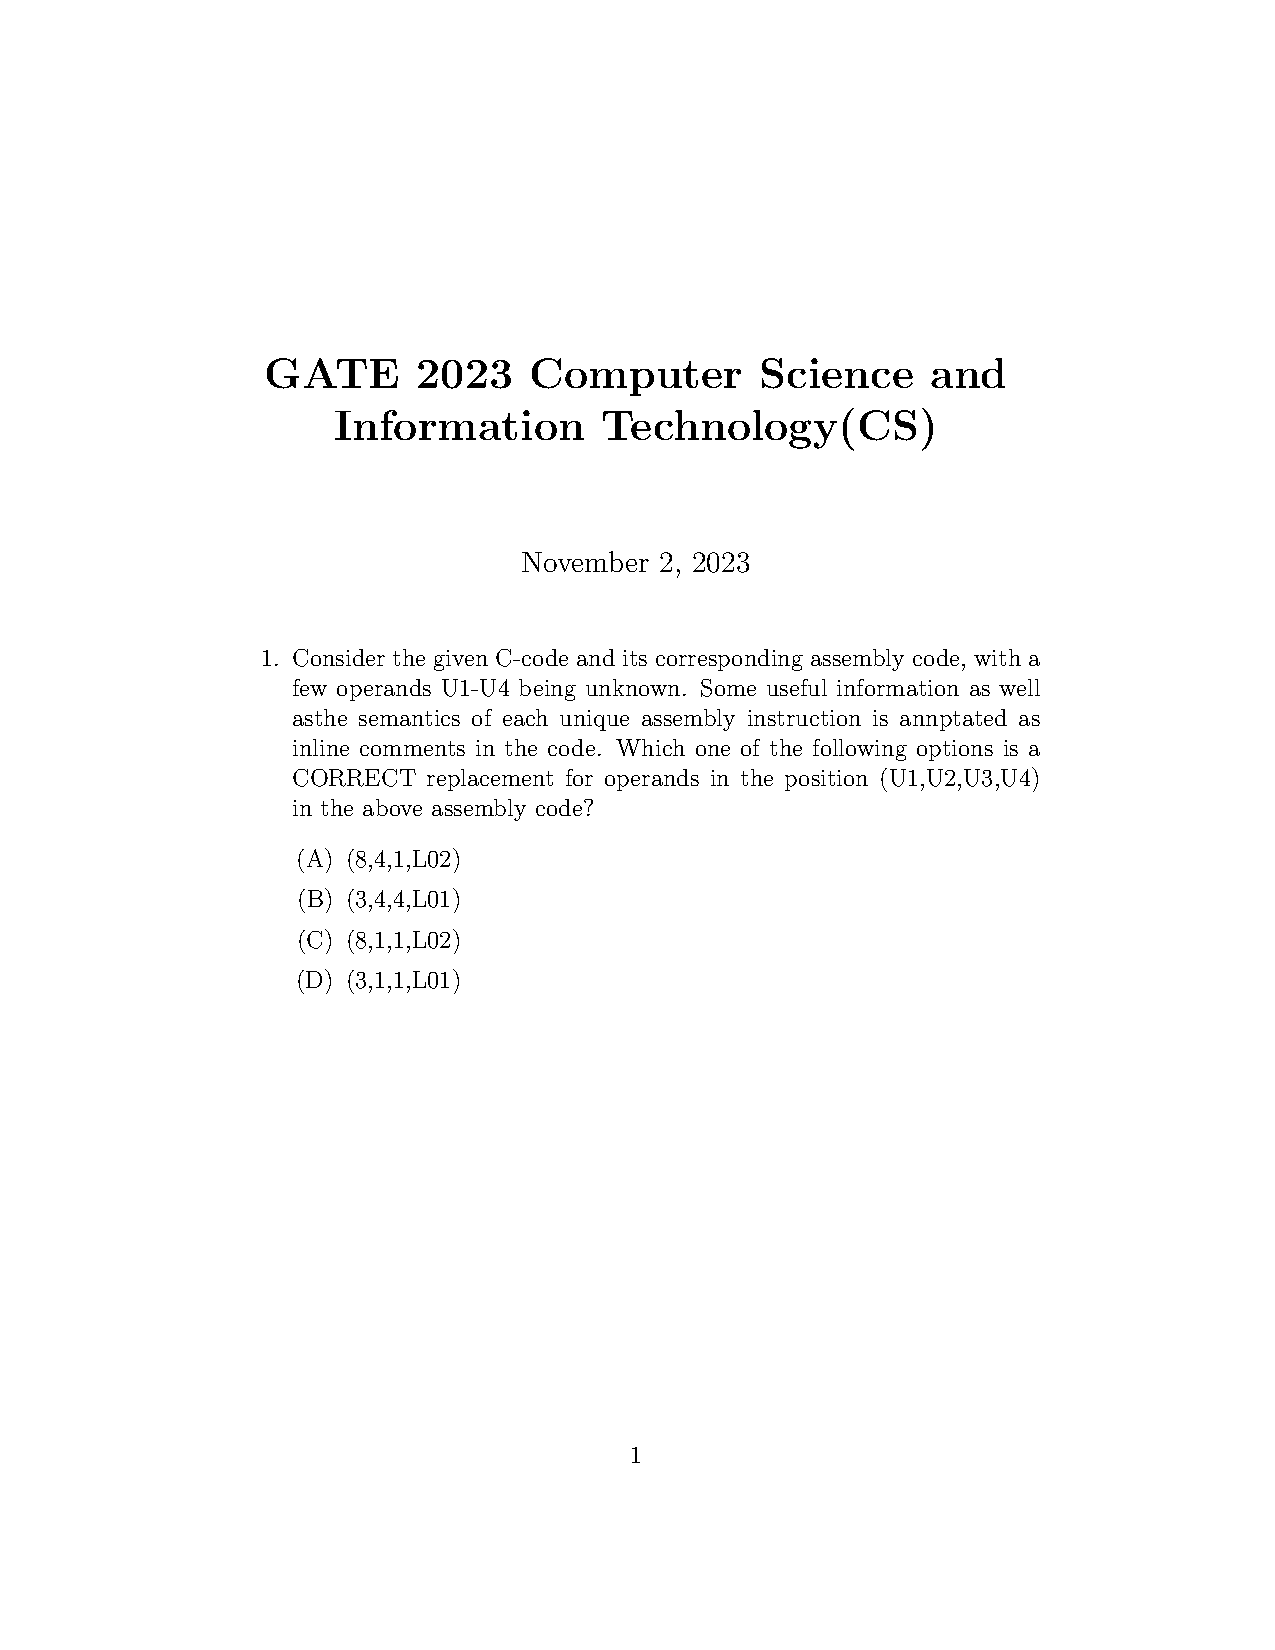
\includegraphics[width=\columnwidth]{/sdcard/FWC/cse.jpg}        
\caption{code}                     \label{fig:code}
\end{figure}

Which one of the following options is a CORRECT replacement for operands in the position (U1,U2,U3,U4) in the above assembly code?

\begin{enumerate}[label=(\Alph*)]  \item (8,4,1,L02)                  \item (3,4,4,L01)
\item (8,1,1,L02)                  \item (3,1,1,L01)                  \end{enumerate}                    \end{enumerate}                    \end{document}
